\documentclass[tikz,svgnames]{standalone}

\usepackage{amsmath,amssymb}

\usetikzlibrary{decorations.markings}

\begin{document}
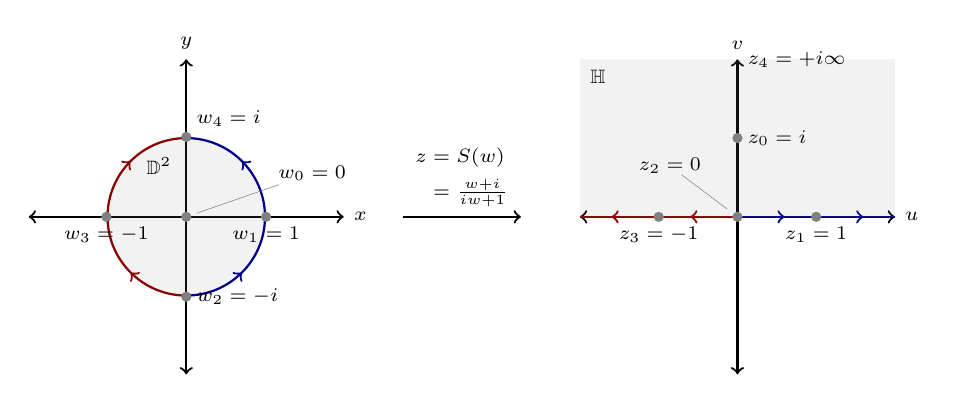
\begin{tikzpicture}[
    thick, font = \scriptsize,
    circ/.style ={circle, fill = gray, draw = gray, inner sep = 1pt}
  ]

  \def\yaxis{2}
  \draw [<->] (-2, 0) -- (2, 0) node (from)[anchor = west]{$x$};
  \draw [<->] (0, -\yaxis) -- (0, \yaxis) node [anchor = south]{$y$};
  \draw [->] (from) (2.75,0) --++(0:1.5) node [anchor = south, midway]{$\begin{aligned}
        z & = S(w) \\
          & =\textstyle \frac{w + i}{i w + 1}
      \end{aligned}$};

  \node (CI) at (0, 0) [circ, fill = gray, opacity = 0.1, minimum size = \yaxis cm]{};

  \begin{scope}[decoration={
          markings,
          mark=at position 0.25 with {\arrow{>}},
          mark=at position 0.75 with {\arrow{>}}}
    ]
    \draw[DarkBlue,postaction={decorate}] (0,-1) arc (-90:90:1);
    \draw[DarkRed,postaction={decorate}] (0,-1) arc (270:90:1);
  \end{scope}

  \node [pin={[pin distance=30,inner sep=1pt]20:$w_0 = 0$}] {};
  \node at (CI.east) [anchor = north] {$w_1 = 1$};
  \node at (CI.south) [anchor = west] {$w_2 = -i$};
  \node at (CI.west) [anchor = north] {$w_3 = -1$};
  \node at (CI.north) [anchor = south west] {$w_4 = i$};
  \node at (CI.110) [anchor = north east, below = 2pt]{$\mathbb{D}^2$};

  \foreach \x in {west, center, east, south, north}{
      \node [circ] at (CI.\x) {};
    };

  \begin{scope}[xshift = 7cm]
    \draw [<->] (-\yaxis, 0) -- (\yaxis, 0) node [anchor = west,text = black]{$u$};
    \draw [<->] (0, -\yaxis) -- (0, \yaxis) node [anchor = south] {$v$};

    \begin{scope}[decoration={
            markings,
            mark=at position 0.3 with {\arrow{>}},
            mark=at position 0.8 with {\arrow{>}}}
      ]
      \draw[DarkRed,postaction={decorate}] (0,0) -- (-2,0);
      \draw[DarkBlue,postaction={decorate}] (0,0) -- (2,0);
    \end{scope}

    \node at (0,1) [anchor = west]{$z_0 = i$};
    \node at (1,0) [anchor = north]{$z_1 = 1$};
    \node [pin={[pin distance=15,inner sep=0pt]130:$z_2 = 0$}] {};
    \node at (-1,0) [anchor = north]{$z_3 = -1$};
    \node at (0,2) [anchor = west]{$z_4 = +i \infty$};
    \node at (0, 1) [circ]{};
    \foreach \x in {-1, 0, 1}{
        \node at (\x, 0) [circ]{};
      }

    \fill [fill = gray, opacity = 0.1] (-2, 0) rectangle (2, 2);
    \node at (-2, 2) [anchor = north west]{$\mathbb{H}$};
  \end{scope}
\end{tikzpicture}
\end{document}
